% GNUPLOT: LaTeX picture with Postscript
\begingroup
  \makeatletter
  \providecommand\color[2][]{%
    \GenericError{(gnuplot) \space\space\space\@spaces}{%
      Package color not loaded in conjunction with
      terminal option `colourtext'%
    }{See the gnuplot documentation for explanation.%
    }{Either use 'blacktext' in gnuplot or load the package
      color.sty in LaTeX.}%
    \renewcommand\color[2][]{}%
  }%
  \providecommand\includegraphics[2][]{%
    \GenericError{(gnuplot) \space\space\space\@spaces}{%
      Package graphicx or graphics not loaded%
    }{See the gnuplot documentation for explanation.%
    }{The gnuplot epslatex terminal needs graphicx.sty or graphics.sty.}%
    \renewcommand\includegraphics[2][]{}%
  }%
  \providecommand\rotatebox[2]{#2}%
  \@ifundefined{ifGPcolor}{%
    \newif\ifGPcolor
    \GPcolorfalse
  }{}%
  \@ifundefined{ifGPblacktext}{%
    \newif\ifGPblacktext
    \GPblacktexttrue
  }{}%
  % define a \g@addto@macro without @ in the name:
  \let\gplgaddtomacro\g@addto@macro
  % define empty templates for all commands taking text:
  \gdef\gplfronttext{}%
  \gdef\gplfronttext{}%
  \makeatother
  \ifGPblacktext
    % no textcolor at all
    \def\colorrgb#1{}%
    \def\colorgray#1{}%
  \else
    % gray or color?
    \ifGPcolor
      \def\colorrgb#1{\color[rgb]{#1}}%
      \def\colorgray#1{\color[gray]{#1}}%
      \expandafter\def\csname LTw\endcsname{\color{white}}%
      \expandafter\def\csname LTb\endcsname{\color{black}}%
      \expandafter\def\csname LTa\endcsname{\color{black}}%
      \expandafter\def\csname LT0\endcsname{\color[rgb]{1,0,0}}%
      \expandafter\def\csname LT1\endcsname{\color[rgb]{0,1,0}}%
      \expandafter\def\csname LT2\endcsname{\color[rgb]{0,0,1}}%
      \expandafter\def\csname LT3\endcsname{\color[rgb]{1,0,1}}%
      \expandafter\def\csname LT4\endcsname{\color[rgb]{0,1,1}}%
      \expandafter\def\csname LT5\endcsname{\color[rgb]{1,1,0}}%
      \expandafter\def\csname LT6\endcsname{\color[rgb]{0,0,0}}%
      \expandafter\def\csname LT7\endcsname{\color[rgb]{1,0.3,0}}%
      \expandafter\def\csname LT8\endcsname{\color[rgb]{0.5,0.5,0.5}}%
    \else
      % gray
      \def\colorrgb#1{\color{black}}%
      \def\colorgray#1{\color[gray]{#1}}%
      \expandafter\def\csname LTw\endcsname{\color{white}}%
      \expandafter\def\csname LTb\endcsname{\color{black}}%
      \expandafter\def\csname LTa\endcsname{\color{black}}%
      \expandafter\def\csname LT0\endcsname{\color{black}}%
      \expandafter\def\csname LT1\endcsname{\color{black}}%
      \expandafter\def\csname LT2\endcsname{\color{black}}%
      \expandafter\def\csname LT3\endcsname{\color{black}}%
      \expandafter\def\csname LT4\endcsname{\color{black}}%
      \expandafter\def\csname LT5\endcsname{\color{black}}%
      \expandafter\def\csname LT6\endcsname{\color{black}}%
      \expandafter\def\csname LT7\endcsname{\color{black}}%
      \expandafter\def\csname LT8\endcsname{\color{black}}%
    \fi
  \fi
  \setlength{\unitlength}{0.02500bp}%
  \begin{picture}(10000.00,4000.00)%
    \gplgaddtomacro\gplfronttext{%
      \colorrgb{0.00,0.00,0.00}%
      \put(1168,736){\makebox(0,0)[r]{\strut{} \scriptsize $0.03$}}%
      \colorrgb{0.00,0.00,0.00}%
      \put(1168,1107){\makebox(0,0)[r]{\strut{}\scriptsize $0.04$}}%
      \colorrgb{0.00,0.00,0.00}%
      \put(1168,1477){\makebox(0,0)[r]{\strut{}\scriptsize $0.05$}}%
      \colorrgb{0.00,0.00,0.00}%
      \put(1168,1847){\makebox(0,0)[r]{\strut{}\scriptsize $0.06$}}%
      \colorrgb{0.00,0.00,0.00}%
      \put(1168,2218){\makebox(0,0)[r]{\strut{}\scriptsize $0.07$}}%
      \colorrgb{0.00,0.00,0.00}%
      \put(1168,2588){\makebox(0,0)[r]{\strut{}\scriptsize $0.08$}}%
      \colorrgb{0.00,0.00,0.00}%
      \put(1168,2958){\makebox(0,0)[r]{\strut{}\scriptsize $0.09$}}%
      \colorrgb{0.00,0.00,0.00}%
      \put(1168,3329){\makebox(0,0)[r]{\strut{}\scriptsize $0.10$}}%
      \colorrgb{0.00,0.00,0.00}%
      \put(1168,3699){\makebox(0,0)[r]{\strut{}\scriptsize $0.11$}}%
      \colorrgb{0.00,0.00,0.00}%
      \put(1625,220){\makebox(0,0){\strut{}\tiny $100\%$}}%
      \colorrgb{0.00,0.00,0.00}%
      \put(2493,220){\makebox(0,0){\strut{}\tiny $>\hspace{-0.1cm}\overline{W}$}}%
      \colorrgb{0.00,0.00,0.00}%
      \put(3361,220){\makebox(0,0){\strut{}\tiny $10\%$}}%
      \colorrgb{0.00,0.00,0.00}%
      \put(4229,220){\makebox(0,0){\strut{}\tiny top}}%
      \colorrgb{0.00,0.00,0.00}%
      %\put(398,2069){\rotatebox{90}{\makebox(0,0){\strut{}$\overline{\|e\|_{2,i}}$, $i = \{1,2,\dots,N\}$}}}%
      \put(-98,2069){\rotatebox{90}{\makebox(0,0){\strut{} \footnotesize WAREHOUSE}}}%
      %\colorrgb{0.00,0.00,0.00}%
      \put(2927,-210){\makebox(0,0){\strut{}\scriptsize Μέθοδος διαλογής}}%
      %\colorrgb{0.00,0.00,0.00}%
      %\put(2927,4029){\makebox(0,0){\strut{}Κατανομή μέσων σφαλμάτων εκτίμησης στάσης ανά μέθοδο επιλογής σωματιδίων}}%
    }%
    \gplgaddtomacro\gplfronttext{%
    }%
    \gplgaddtomacro\gplfronttext{%
      \colorrgb{0.00,0.00,0.00}%
      \put(5663,440){\makebox(0,0)[r]{\strut{} \scriptsize $0.025$}}%
      \colorrgb{0.00,0.00,0.00}%
      \put(5663,934){\makebox(0,0)[r]{\strut{}\scriptsize $0.030$}}%
      \colorrgb{0.00,0.00,0.00}%
      \put(5663,1428){\makebox(0,0)[r]{\strut{}\scriptsize $0.035$}}%
      \colorrgb{0.00,0.00,0.00}%
      \put(5663,1921){\makebox(0,0)[r]{\strut{}\scriptsize $0.040$}}%
      \colorrgb{0.00,0.00,0.00}%
      \put(5663,2415){\makebox(0,0)[r]{\strut{}\scriptsize $0.045$}}%
      \colorrgb{0.00,0.00,0.00}%
      \put(5663,2909){\makebox(0,0)[r]{\strut{}\scriptsize $0.050$}}%
      \colorrgb{0.00,0.00,0.00}%
      \put(5663,3403){\makebox(0,0)[r]{\strut{}\scriptsize $0.055$}}%
      \colorrgb{0.00,0.00,0.00}%
      \put(6120,220){\makebox(0,0){\strut{}\tiny $100\%$}}%
      \colorrgb{0.00,0.00,0.00}%
      \put(6988,220){\makebox(0,0){\strut{}\tiny $>\hspace{-0.1cm}\overline{W}$}}%
      \colorrgb{0.00,0.00,0.00}%
      \put(7856,220){\makebox(0,0){\strut{}\tiny $10\%$}}%
      \colorrgb{0.00,0.00,0.00}%
      \put(8724,220){\makebox(0,0){\strut{}\tiny top}}%
      \colorrgb{0.00,0.00,0.00}%
      \put(7422,-210){\makebox(0,0){\strut{}\scriptsize Μέθοδος διαλογής}}%
      %\colorrgb{0.00,0.00,0.00}%
      %\put(7422,4029){\makebox(0,0){\strut{}WAREHOUSE pose errors per pose selection method}}%
    }%
    \gplgaddtomacro\gplfronttext{%
    }%
    \put(0,0){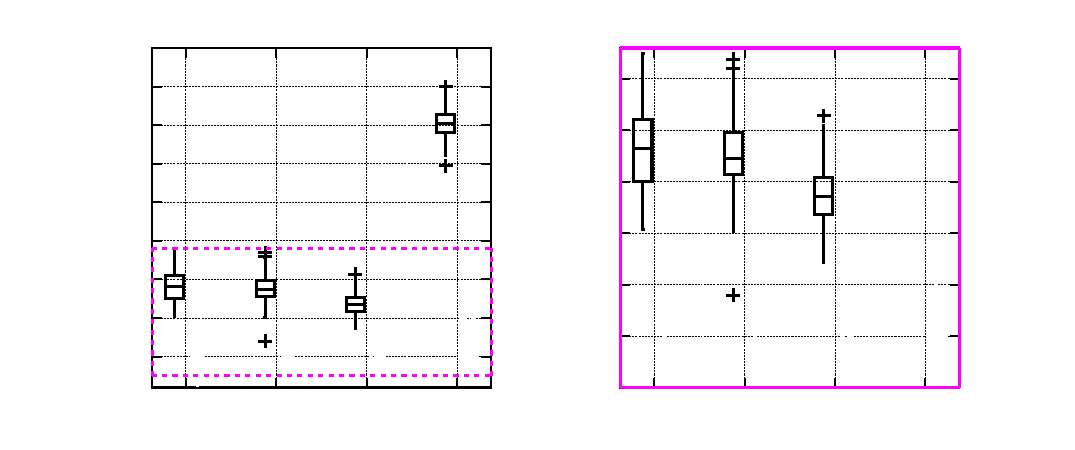
\includegraphics[scale=0.5]{./figures/slides/ch4/experiments/boxplots/warehouse_mean_total_errors_per_selection}}%
    \gplfronttext
  \end{picture}%
\endgroup
